
%(BEGIN_QUESTION)
% Copyright 2015, Tony R. Kuphaldt, released under the Creative Commons Attribution License (v 1.0)
% This means you may do almost anything with this work of mine, so long as you give me proper credit

The level transmitter (LT-31) on vessel V-5 failed at 1:00 PM today, its signal going all the way to zero even though there was still liquid inside the vessel.  You are asked to calculate the amount of liquid in the vessel at 3:00 PM based on the flow trends shown (in units of gallons per {\it hour}):

$$\includegraphics[width=15.5cm]{i02886x01.eps}$$

$V$ @ 3:00 PM = \underbar{\hskip 50pt} gallons

\vskip 10pt

\underbar{file i02886}
%(END_QUESTION)





%(BEGIN_ANSWER)

We are asked to find the number of {\it gallons} inside the vessel given flow rates in {\it gallons per hour} and time in {\it hours}.  Therefore, the mathematical operation we must employ is multiplication (so that ``hours'' cancels out to leave ``gallons'') and that means {\it integration}.

The vessel's accumulated volume rises or falls according to the difference between the incoming and outgoing flow rates over time.  Mathematically we may express this by the following integral:

$$V = \int_{t_0}^{t_f} (Q_{in} - Q_{out}) \> dt + V_0$$

The level transmitter stopped working at 1:00 PM, so the last known volume of liquid inside the tank was measured then: 22.5 gallons.  This must then be our initial volume ($V_0$), with 1:00 PM being the lower limit of our integration interval.  The upper limit of our integration interval must be 3:00 PM which is the time when we're interested in the tank's liquid volume.  Therefore:

$$V_{3:00} = \int_{1:00}^{3:00} (Q_{in} - Q_{out}) \> dt + 22.5 \hbox{ gal}$$

Evaluating this integral graphically, we end up with the following shaded area between the two flowmeter trendlines:

$$\includegraphics[width=15.5cm]{i02886x02.eps}$$

The area of this trapezoid (calculated as the area of a 3x3 square and a 3x6 triangle) is (7.5 gal/hr)(0.5 hr) + (0.5)(7.5 gal/hr)(1 hr) = 7.5 gallons.  Thus:

$$V_{3:00} = \int_{1:00}^{3:00} (Q_{in} - Q_{out}) \> dt + 22.5 \hbox{ gal}$$

$$V_{3:00} = 7.5 \hbox{ gal} + 22.5 \hbox{ gal} = 30 \hbox{ gal}$$

Vessel V-5 therefore contains 30 gallons of liquid at 3:00 PM.

%(END_ANSWER)





%(BEGIN_NOTES)


%INDEX% Mathematics, calculus: integral (accumulated volume as the integral of flow)
%INDEX% Mathematics, calculus: integration (numerical)

%(END_NOTES)


